\documentclass[12pt, a4paper]{article}%{{{
\usepackage[utf8]{inputenc}
\usepackage[T1]{fontenc}
\usepackage[a4paper,left=2cm,right=2cm,top=2cm,bottom=2cm]{geometry}
\usepackage[frenchb]{babel}
\usepackage{libertine}
\usepackage{float}
\usepackage{hyperref}
\usepackage{amsfonts}
\usepackage{amssymb}
\usepackage[dvipsnames]{xcolor}
\usepackage[pdftex]{graphicx}

\setlength{\parindent}{0cm}
\setlength{\parskip}{1ex plus 0.5ex minus 0.2ex}
\newcommand{\hsp}{\hspace{20pt}}
\newcommand{\HRule}{\rule{\linewidth}{0.5mm}}

\begin{document}

\begin{titlepage}
  \begin{sffamily}
  \begin{center}

    % Upper part of the page. The '~' is needed because \\
    % only works if a paragraph has started.
    
\includegraphics[scale=1]{Images/polytechnique_genie_gauche_fr_rgb.png}~\\[1.5cm]

    \textsc{\LARGE École Polytechnique Montréal}\\[2cm]

    \textsc{\Large INF8405 : Informatique Mobile}\\[1.5cm]

    % Title
    \HRule \\[0.4cm]
    { \huge \bfseries TP1 : FlowFree\\[0.4cm] }

    \HRule \\[2cm]
    
\includegraphics[scale=1]{Images/logoFF.png}\\[2cm]

    % Author and supervisor
    \begin{minipage}{0.4\textwidth}
      \begin{flushleft} \large
          Philippe TROCLET \textsc{1815208}\\
          Alexandre  MAO \textsc{1813566}\\
          Fabien  BERQUEZ \textsc{1800325}\\
      \end{flushleft}
    \end{minipage}
    \begin{minipage}{0.4\textwidth}
      \begin{flushright} \large
        \emph{Soumis à :} M. Aurel Josas RANDOLF\\
        \emph{Soumis le :} 17 Février 2016 
      \end{flushright}
    \end{minipage}

    \vfill

  \end{center}
  \end{sffamily}
\end{titlepage}%}}}


\section{Introduction}
	L'objectif de ce laboratoire était de développer une application permettant de joueur au jeu du Flow free sur Android. Le jeu de Flow free dispose de règles assez simple : des paires de jetons de couleur sont placés sur une grille carrée d'une taille donnée (ici pour notre application, 7x7 ou 8x8). Le joueur doit alors relier chaque paire de jetons de l'un à l'autre, en traçant des tubes avec le doigt. La partie est remportée si les jetons de chaque paire sont reliés, que toutes les cases sont occupées par un tube, et qu'il n'y a aucune superposition de tubes sur une même case. Dans le cas où toutes les cases ne sont pas utilisées, la partie est inachevée. Sinon, la partie est perdue.
	\newline
	Les contraintes techniques sur cette application étaient de pouvoir être utilisée sur les versions d'Android supportant l'API 18 (Android 4.3.1) et plus (jusqu'à 23 pour la version actuelle, Android 6). Le jeu devant être adapté pour des supports mobiles variés (tablettes, téléphones intelligents, ...), il doit de plus être jouable entièrement tactilement. Enfin, l'application doit être la plus facile d'accès possible, et proposer à la fois des comportements intuitifs pour les utilisateurs de dispositifs mobiles, et une navigation facile à travers les différentes options possibles.
	\newline
	Pour respecter ces requis non-fonctionnels, nous avons donc opté pour un certain nombre de considérations d'ergonomie, sur les règles du jeu, sur les possibilités offertes au joueur. Nous allons les examiner dans la section suivante.
	
\section{Présentation générale}
	Nous allons présenter dans cette partie les choix que nous avons réalisés pour offrir aux utilisateurs de l'application une navigation et une expérience de jeu que nous espérons aisées et intuitives.
	
	\subsection{Menus de l'application}
	Nous avons opté pour un menu d'accueil proposant trois options : \textit{démarrer} une partie, accéder aux \textit{instructions} et \textit{quitter} l'application.
	Lorsque l'utilisateur choisit de démarrer la partie, un autre menu s'affiche et lui demande de choisir la taille de la grille, puis, une fois celle-ci choisie, l'utilisateur doit choisir le niveau qu'il va jouer. L'écran de jeu s'affiche alors et le joueur peut débuter. Sur les trois écrans mentionnés, l'utilisateur peut à tout moment quitter l'application en utilisant le menu dans la barre de l'application  (symbolisé sur Android 5 et 6 par les 3 points en haut à droite de la barre) [voir figures \ref{fig:menus} et \ref{fig:quitter}]
	\begin{figure}
	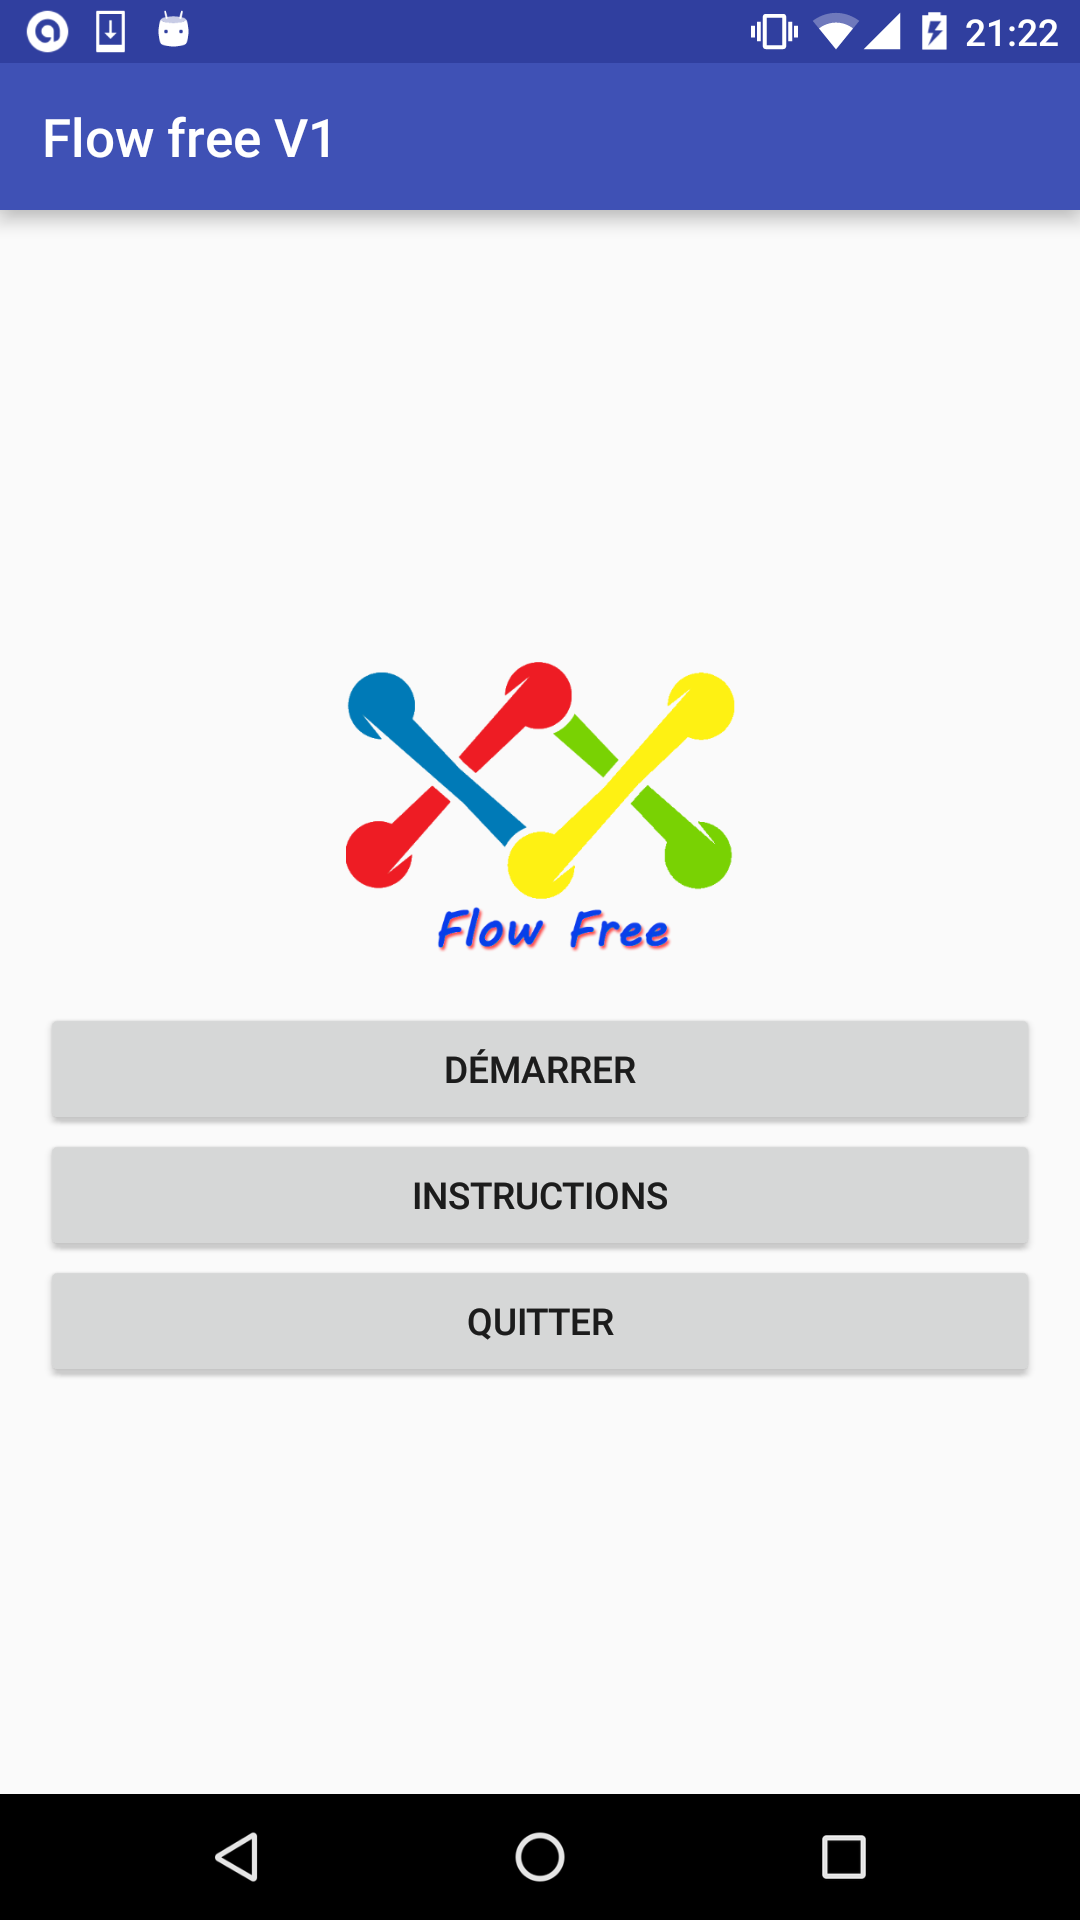
\includegraphics[width=5cm]{Images/nexus_1.png}\hfill
	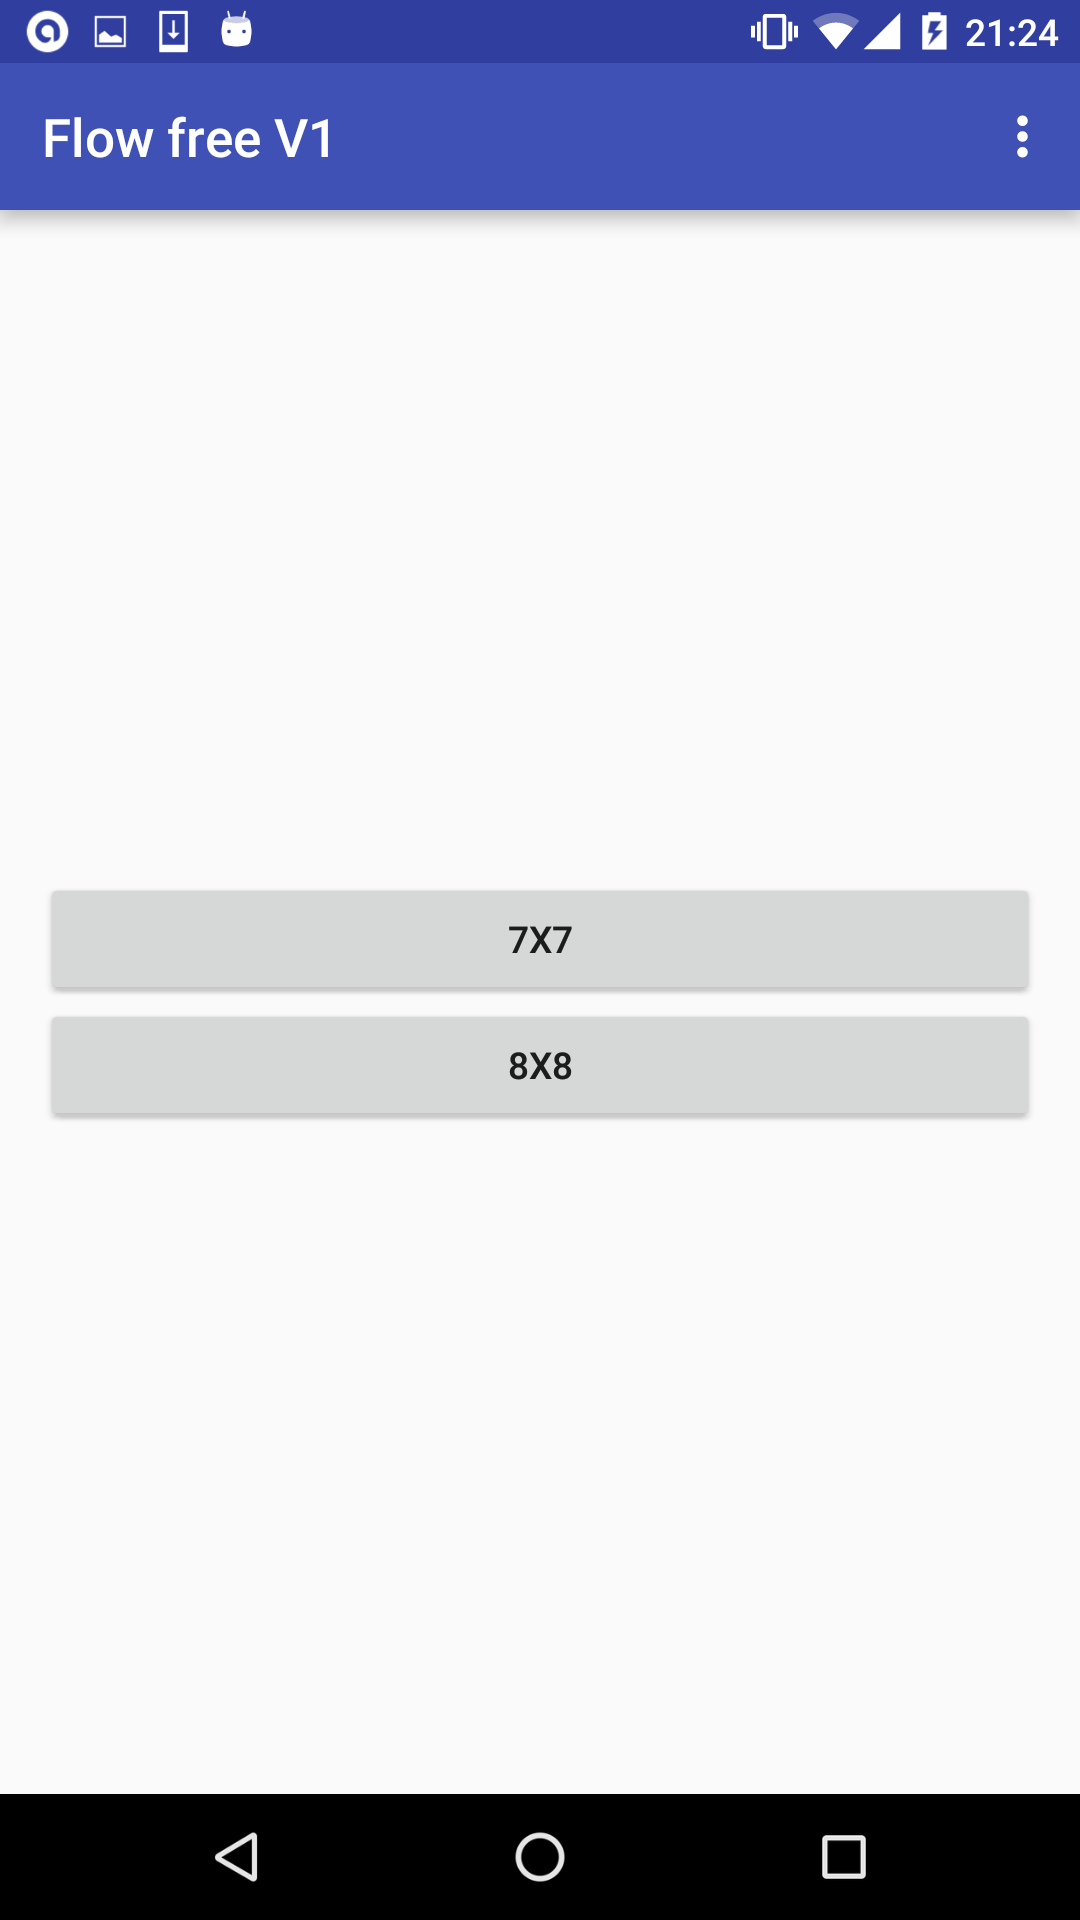
\includegraphics[width=5cm]{Images/nexus_3.png}\hfill
	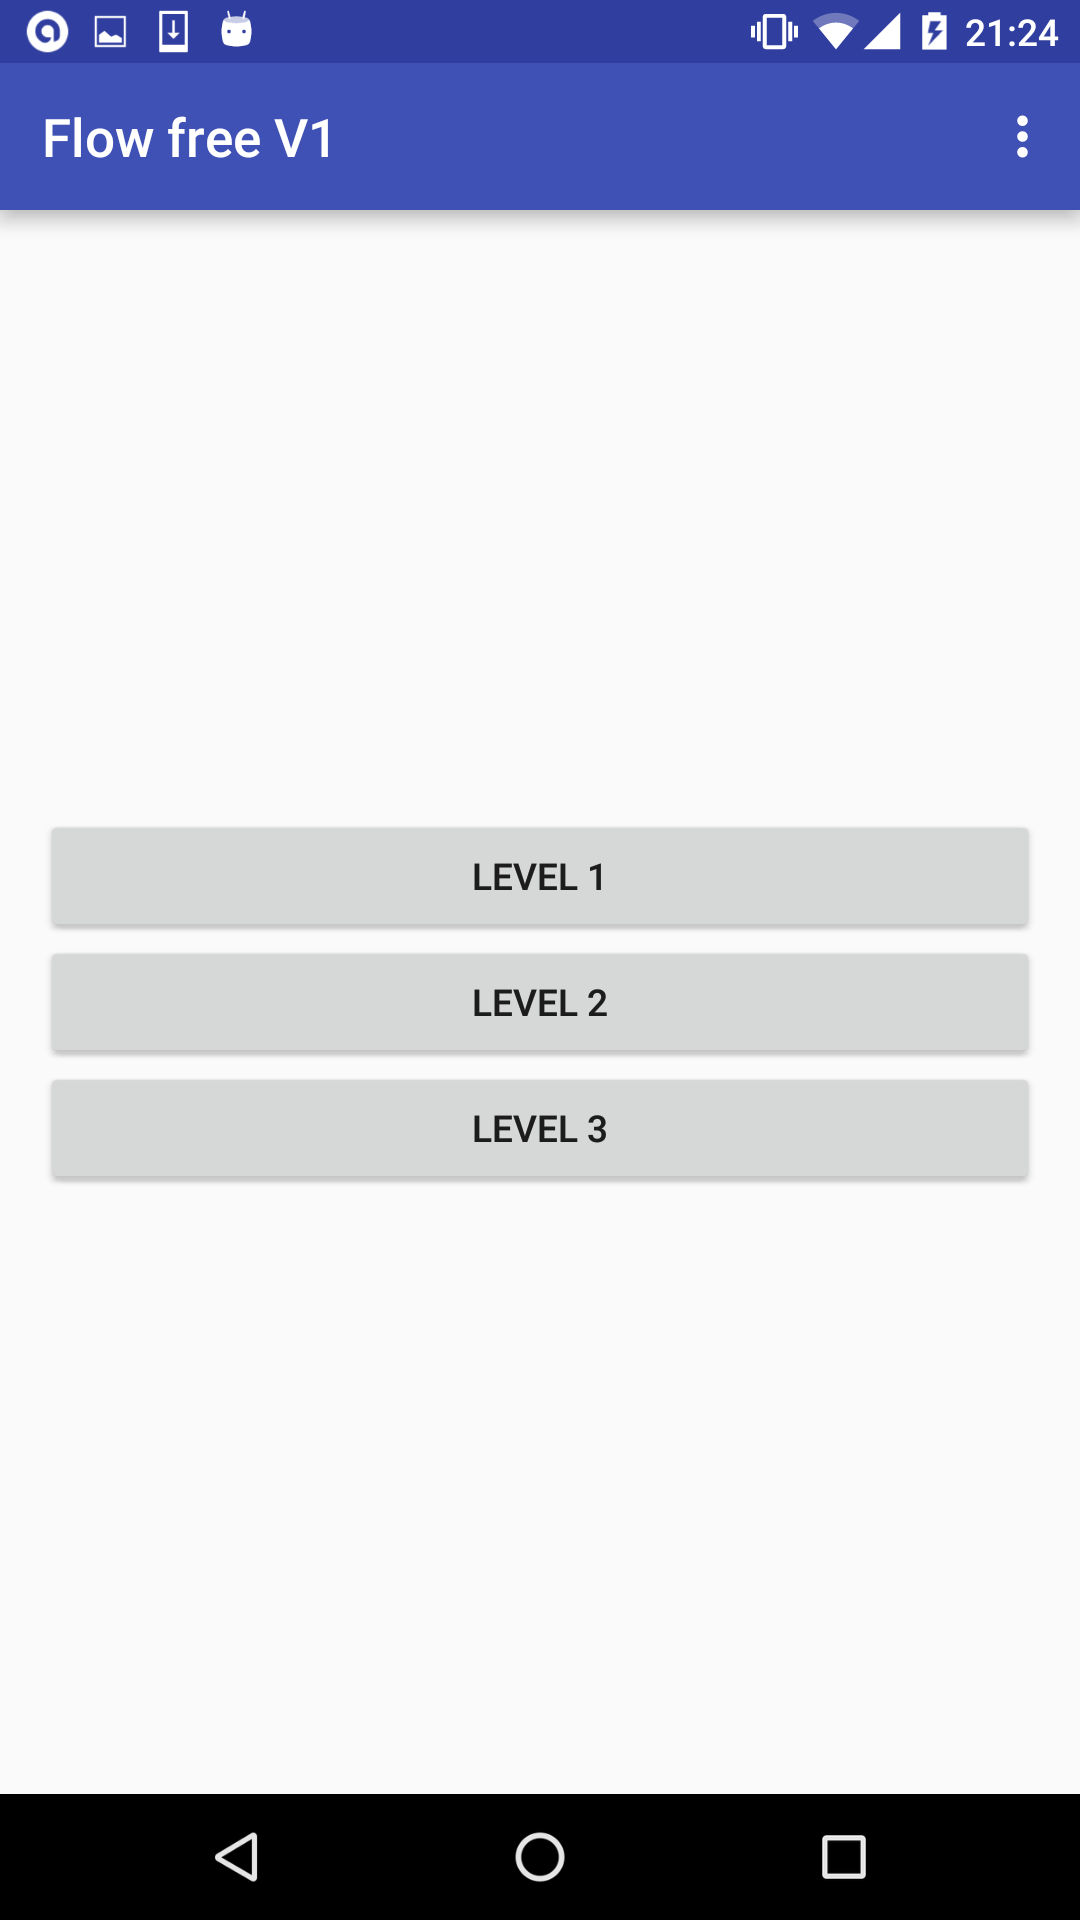
\includegraphics[width=5cm]{Images/nexus_4.png}
	\caption{Menus sur un Google Nexus 5X (Android 6)}\label{fig:menus}
\end{figure}

	\subsection{Quitter l'application}
	Pour empêcher l'utilisateur de quitter de manière involontaire l'application, le choix de quitter dans les différents menus est soumis à une confirmation, qui se fait par l'intermédiaire d'une fenêtre pop-up offrant deux choix de réponses : Oui et Non. [voir figure \ref{fig:quitter}]
	
\begin{figure}
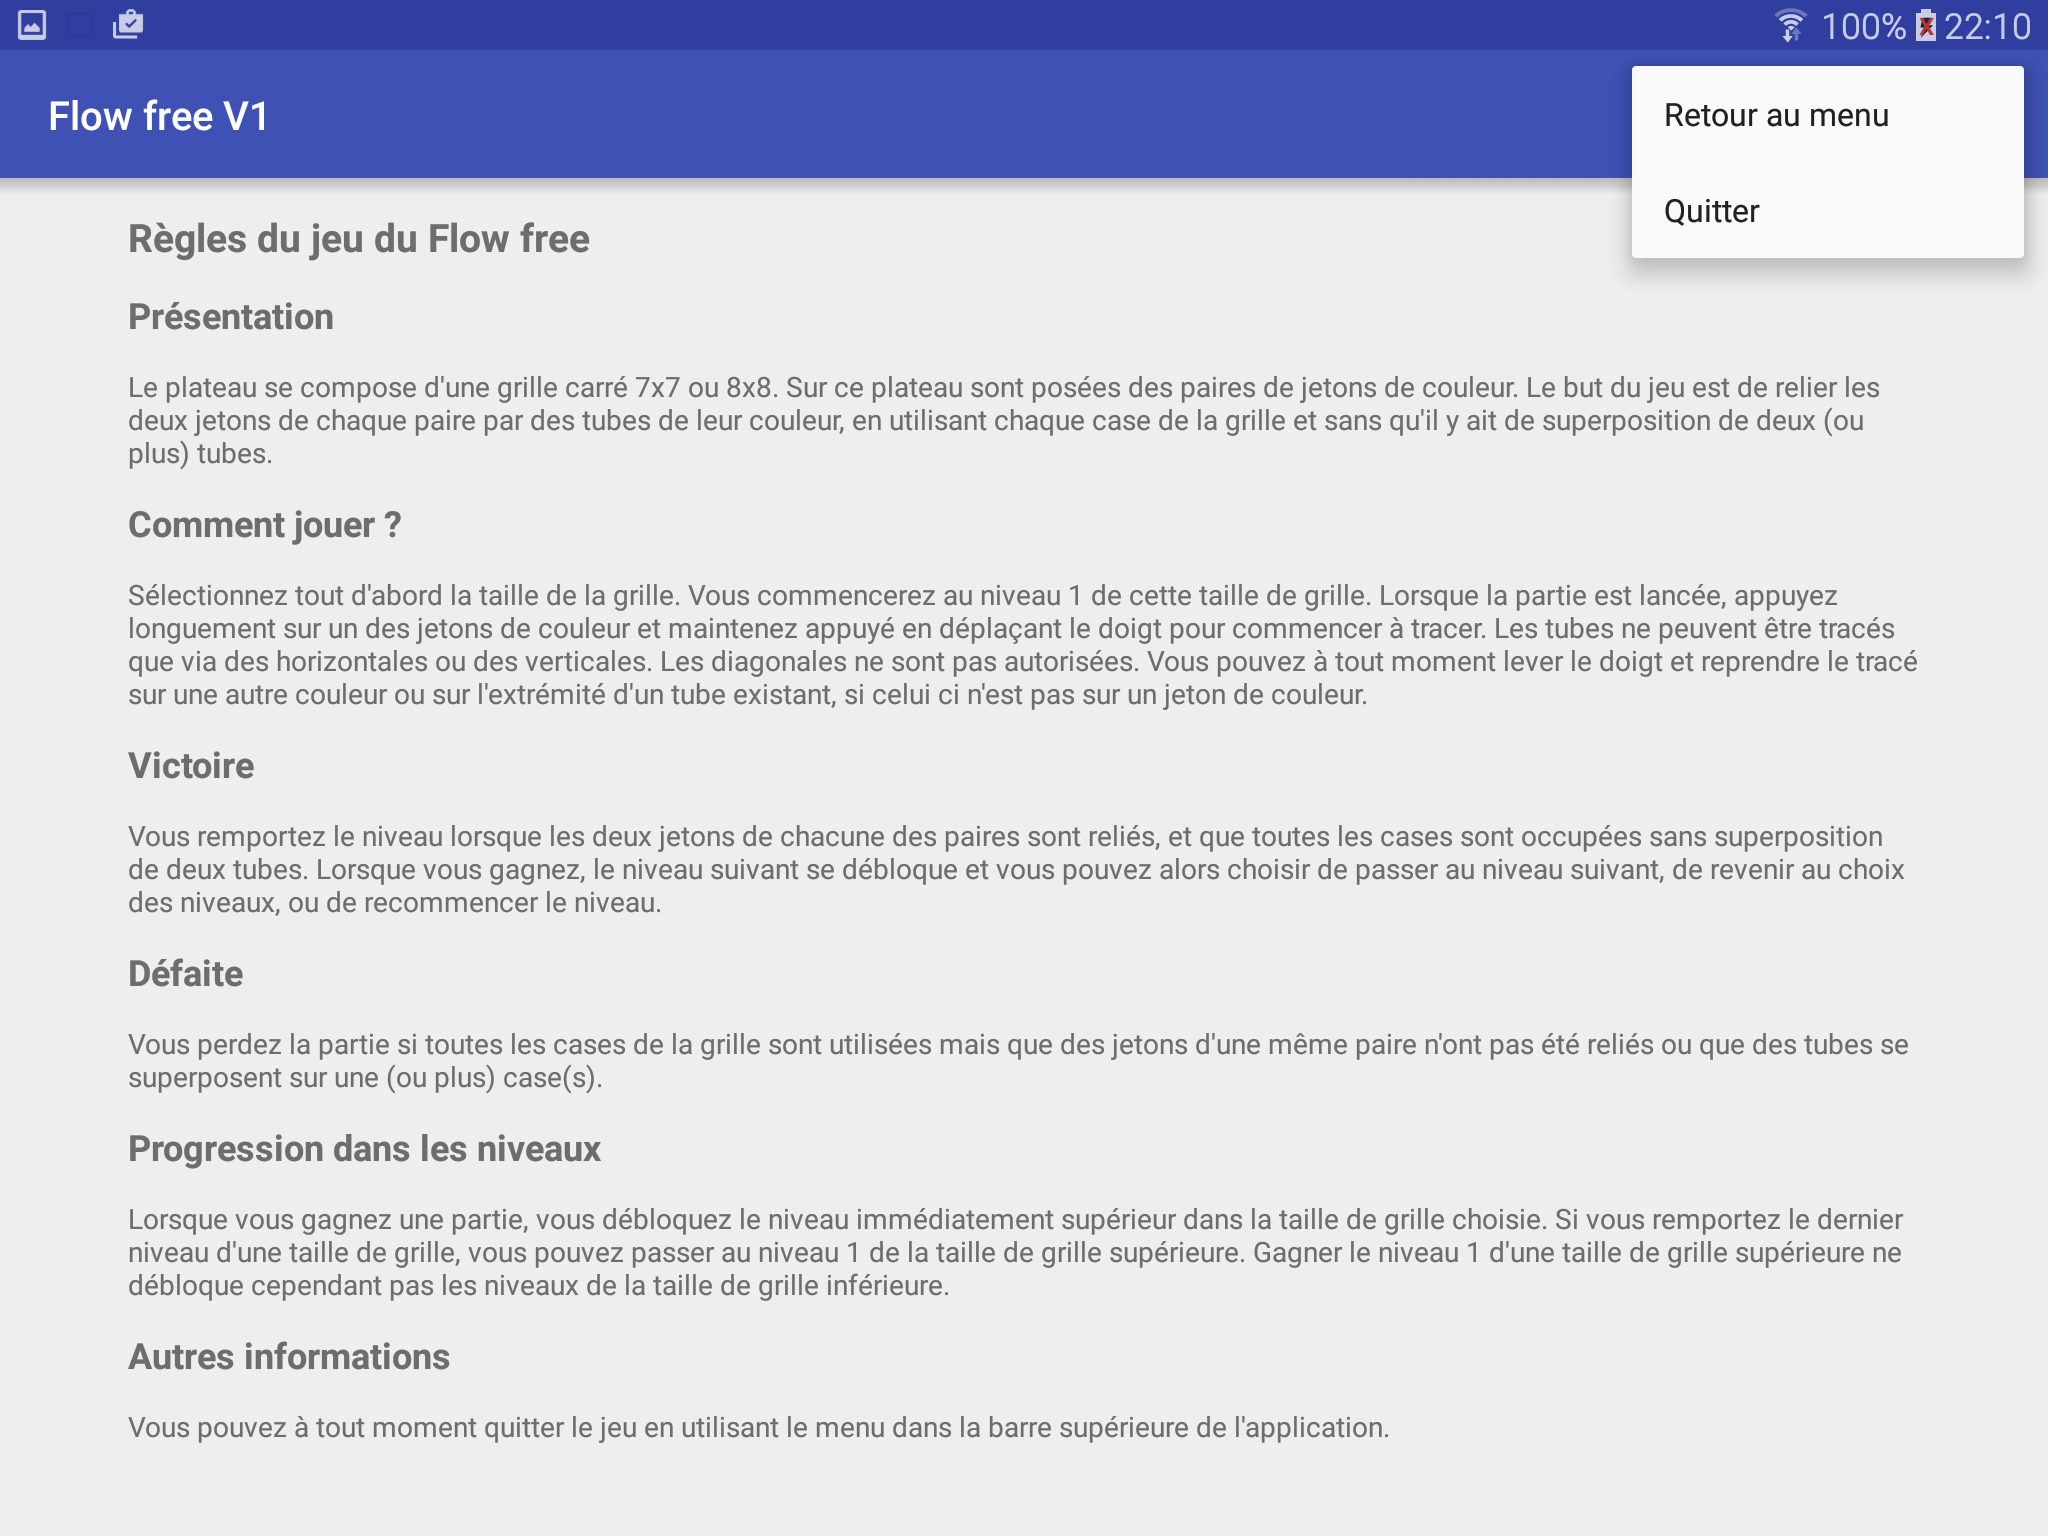
\includegraphics[width=11cm]{Images/s2_2.png}\hfill
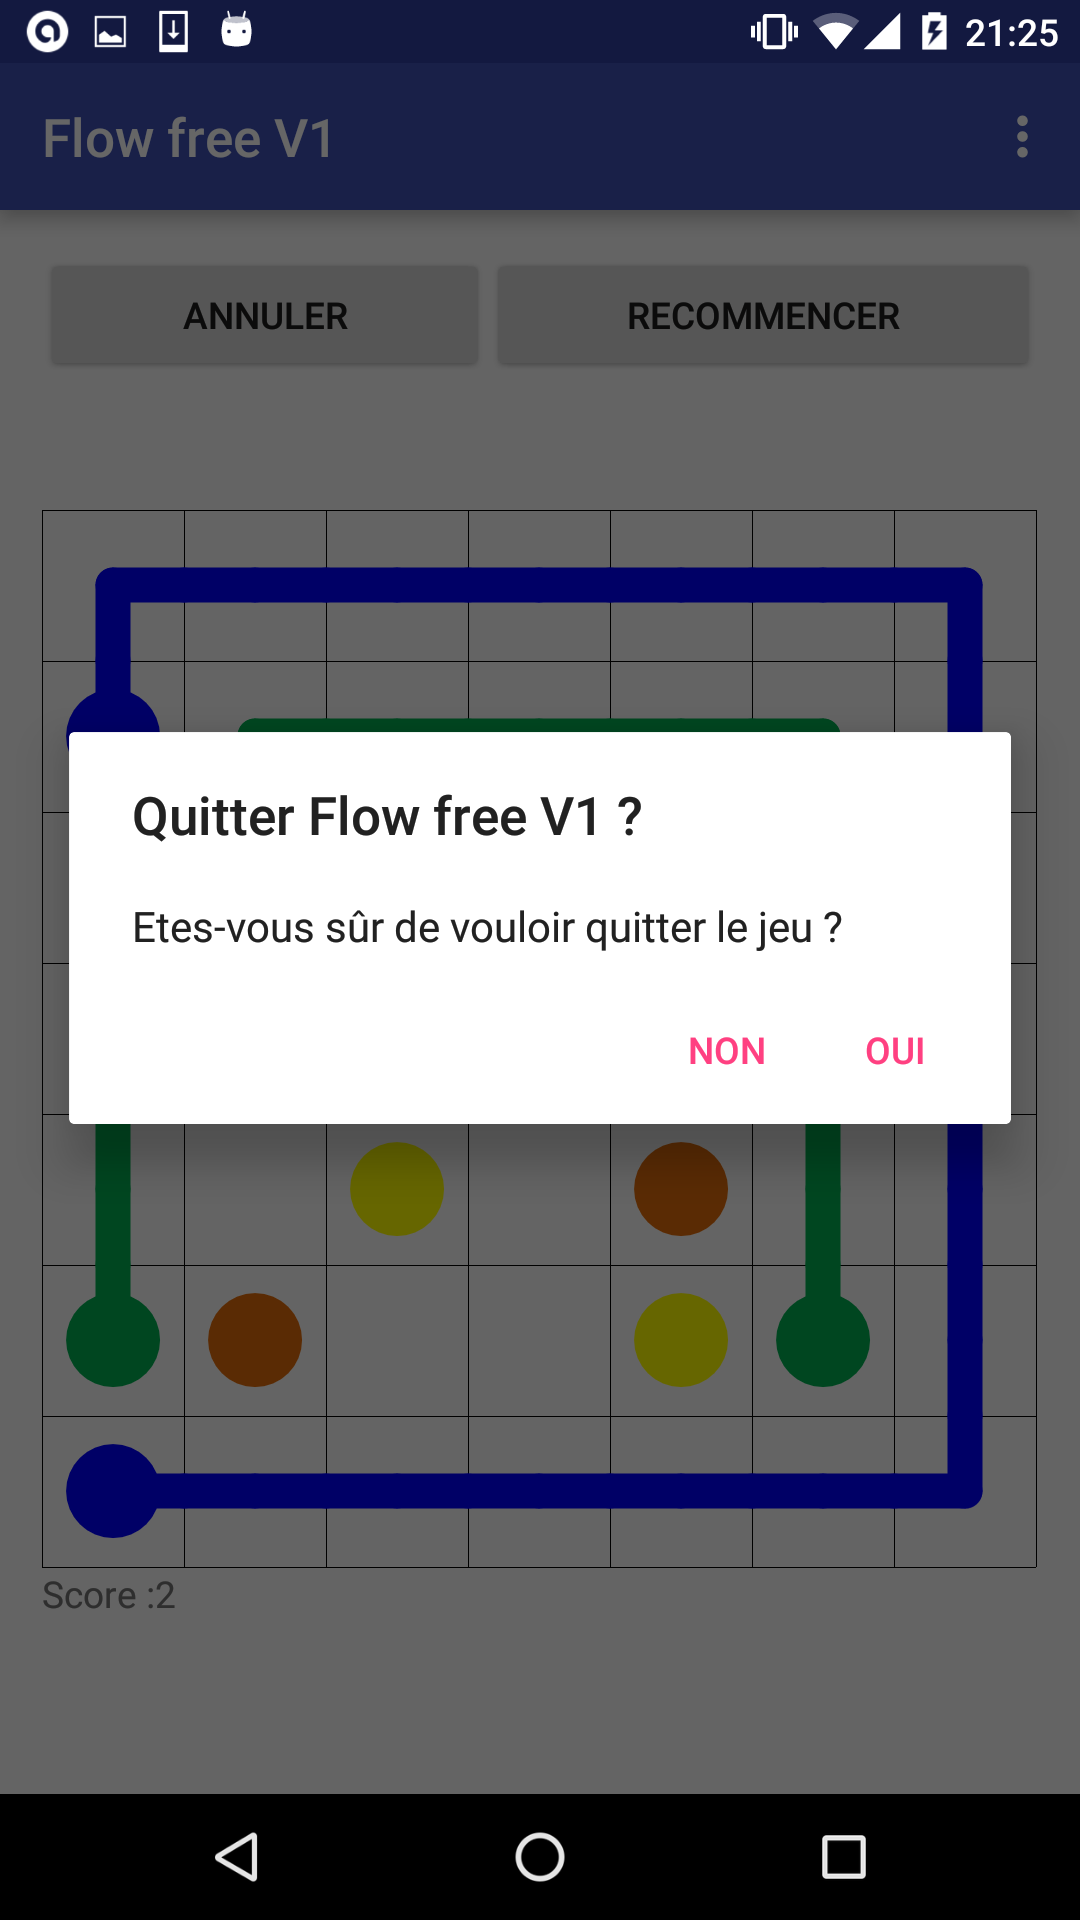
\includegraphics[width=5cm]{Images/nexus_7.png}
\caption{Processus pour quitter sur un Samsung Galaxy Tab 2 et Google Nexus 5X}\label{fig:quitter}
\end{figure}
	
	\subsection{Déroulement du jeu}
	Une fois la partie lancée, les mécanismes impliqués pour que le joueur puisse jouer sont assez commun à beaucoup de jeux, et, nous l'espérons, intuitifs. Le joueur commence à tracer un tube d'une couleur en appuyant le doigt sur le jeton de départ qu'il a choisi, puis en maintenant appuyé pour tracer le tube de la couleur en question. Le tube en formation s'affiche au fur et à mesure que le joueur déplace son doigt. Lorsque le joueur relève le doigt, le tracé s'arrête, mais le joueur à la possibilité de continuer à tout moment le trait qu'il vient d'interrompre en appuyant le doigt sur l'extrémité actuelle du tube. Sinon, il peut passer à un autre jeton de départ (et une autre couleur) ou bien poursuivre un autre tracé.
	\newline
	Afin d'offrir un confort maximal et de permettre au joueur de ne pas avoir à recommencer à chaque erreur de tracé, une fonction d'annulation a été incluse. Elle permet d'effacer du plus récent au plus ancien les derniers morceaux de tubes qui ont été tracés. Une fonction de réinitialisation est également présente pour revenir à la configuration de départ du niveau.
	
	\begin{figure}
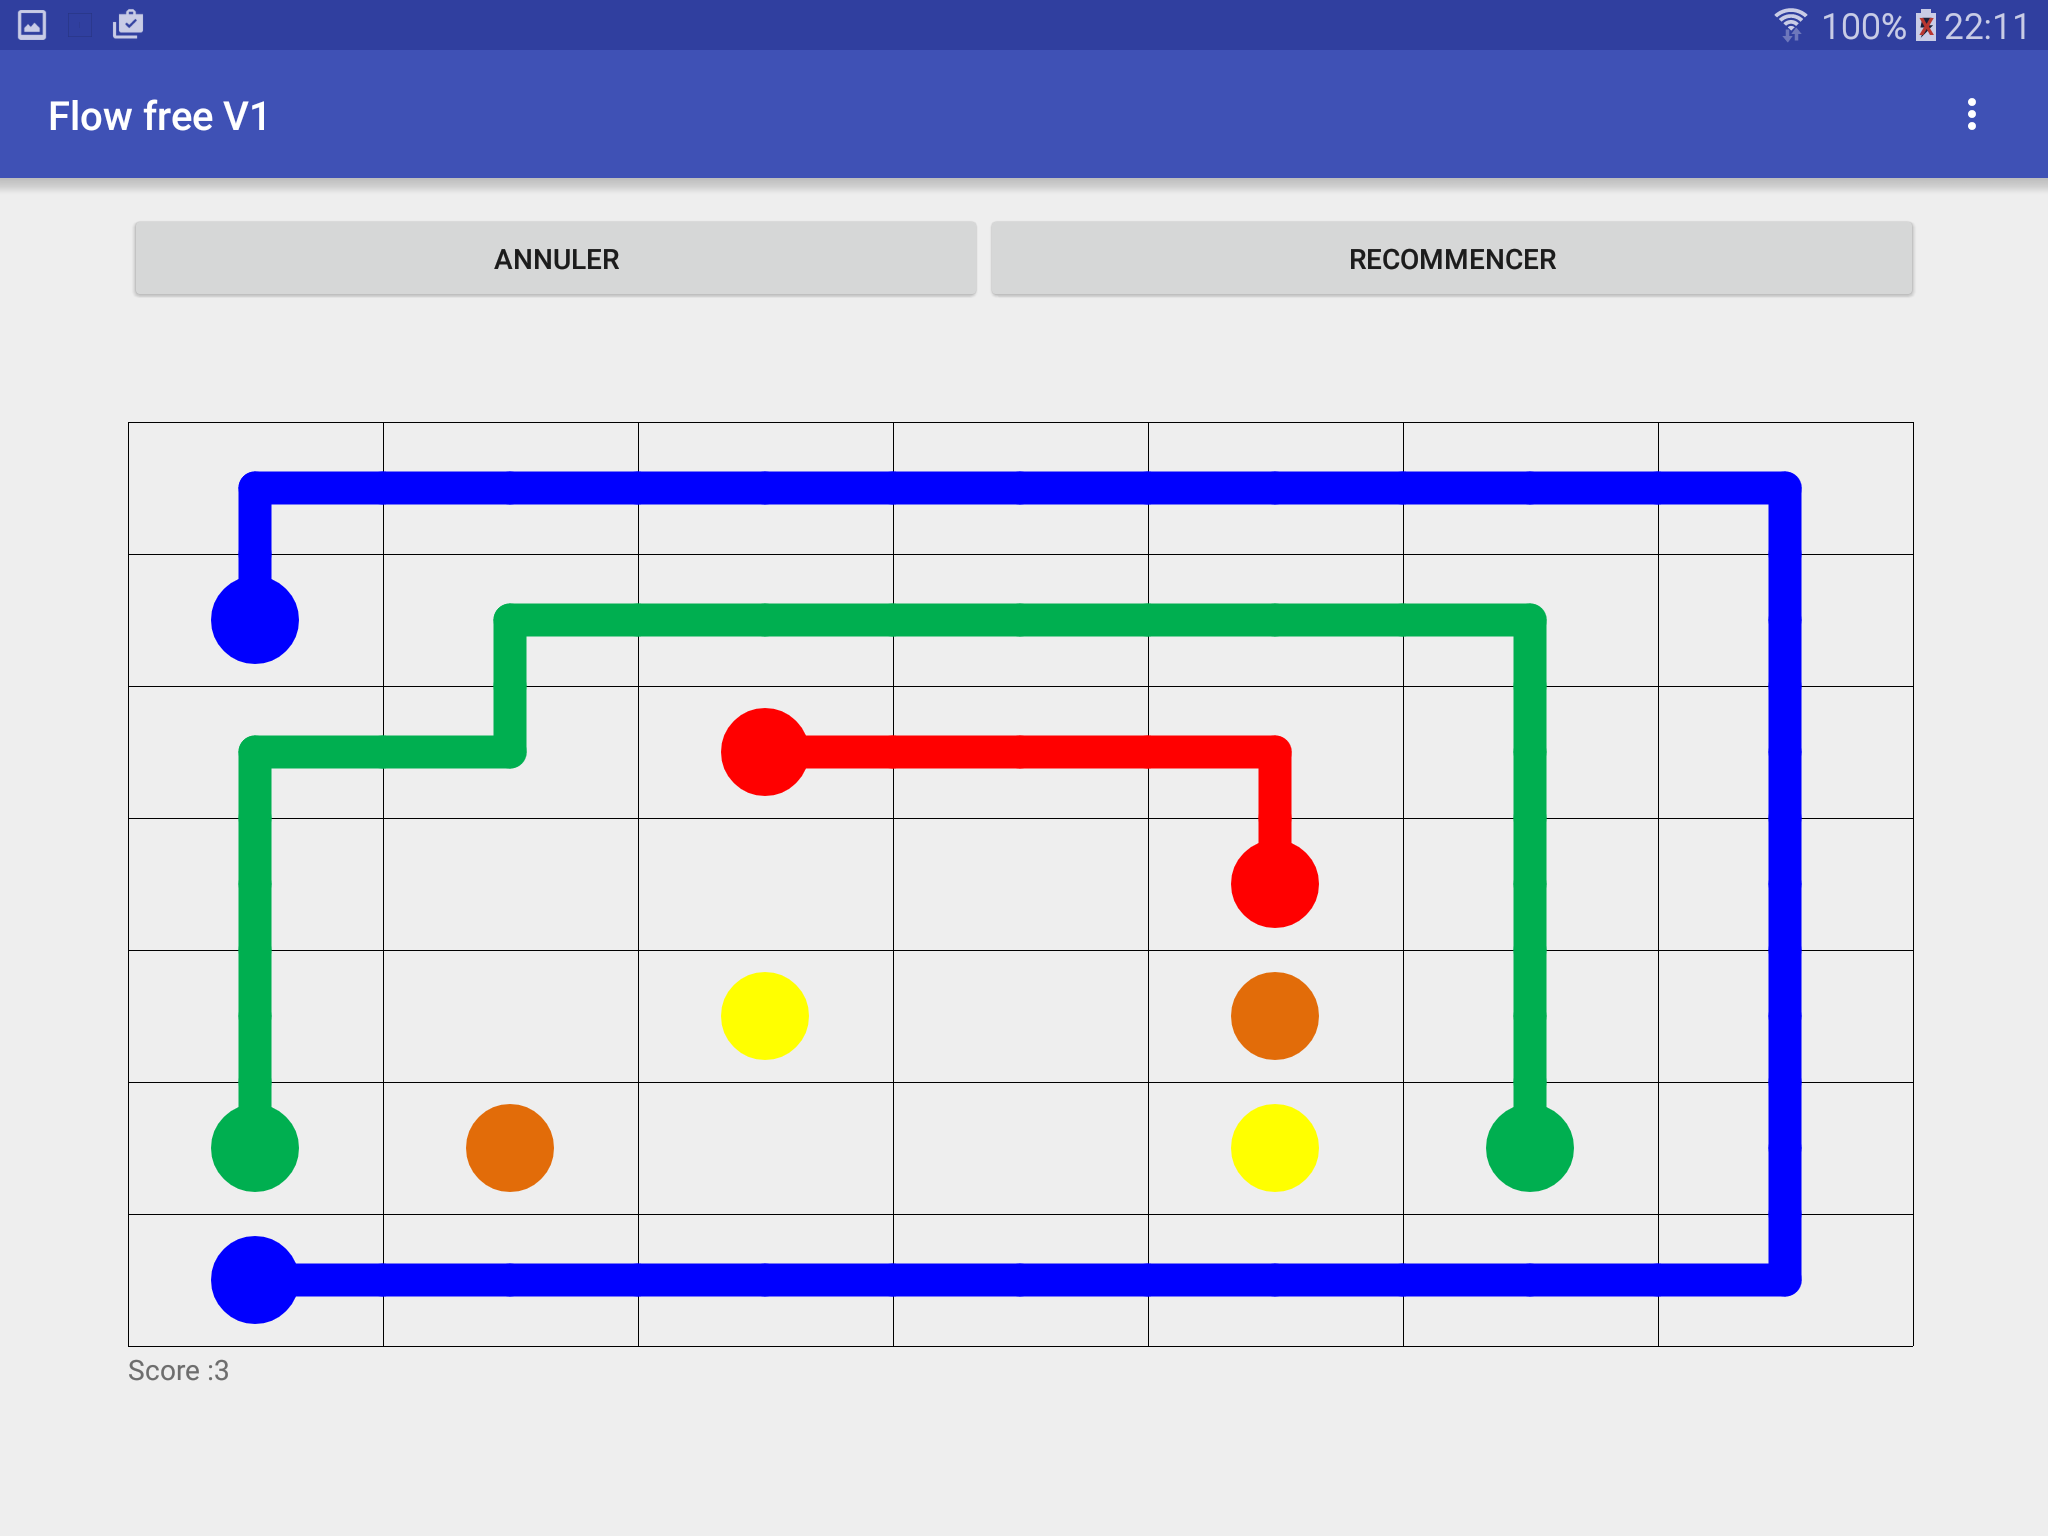
\includegraphics[width=8cm]{Images/s2_3.png}\hfill
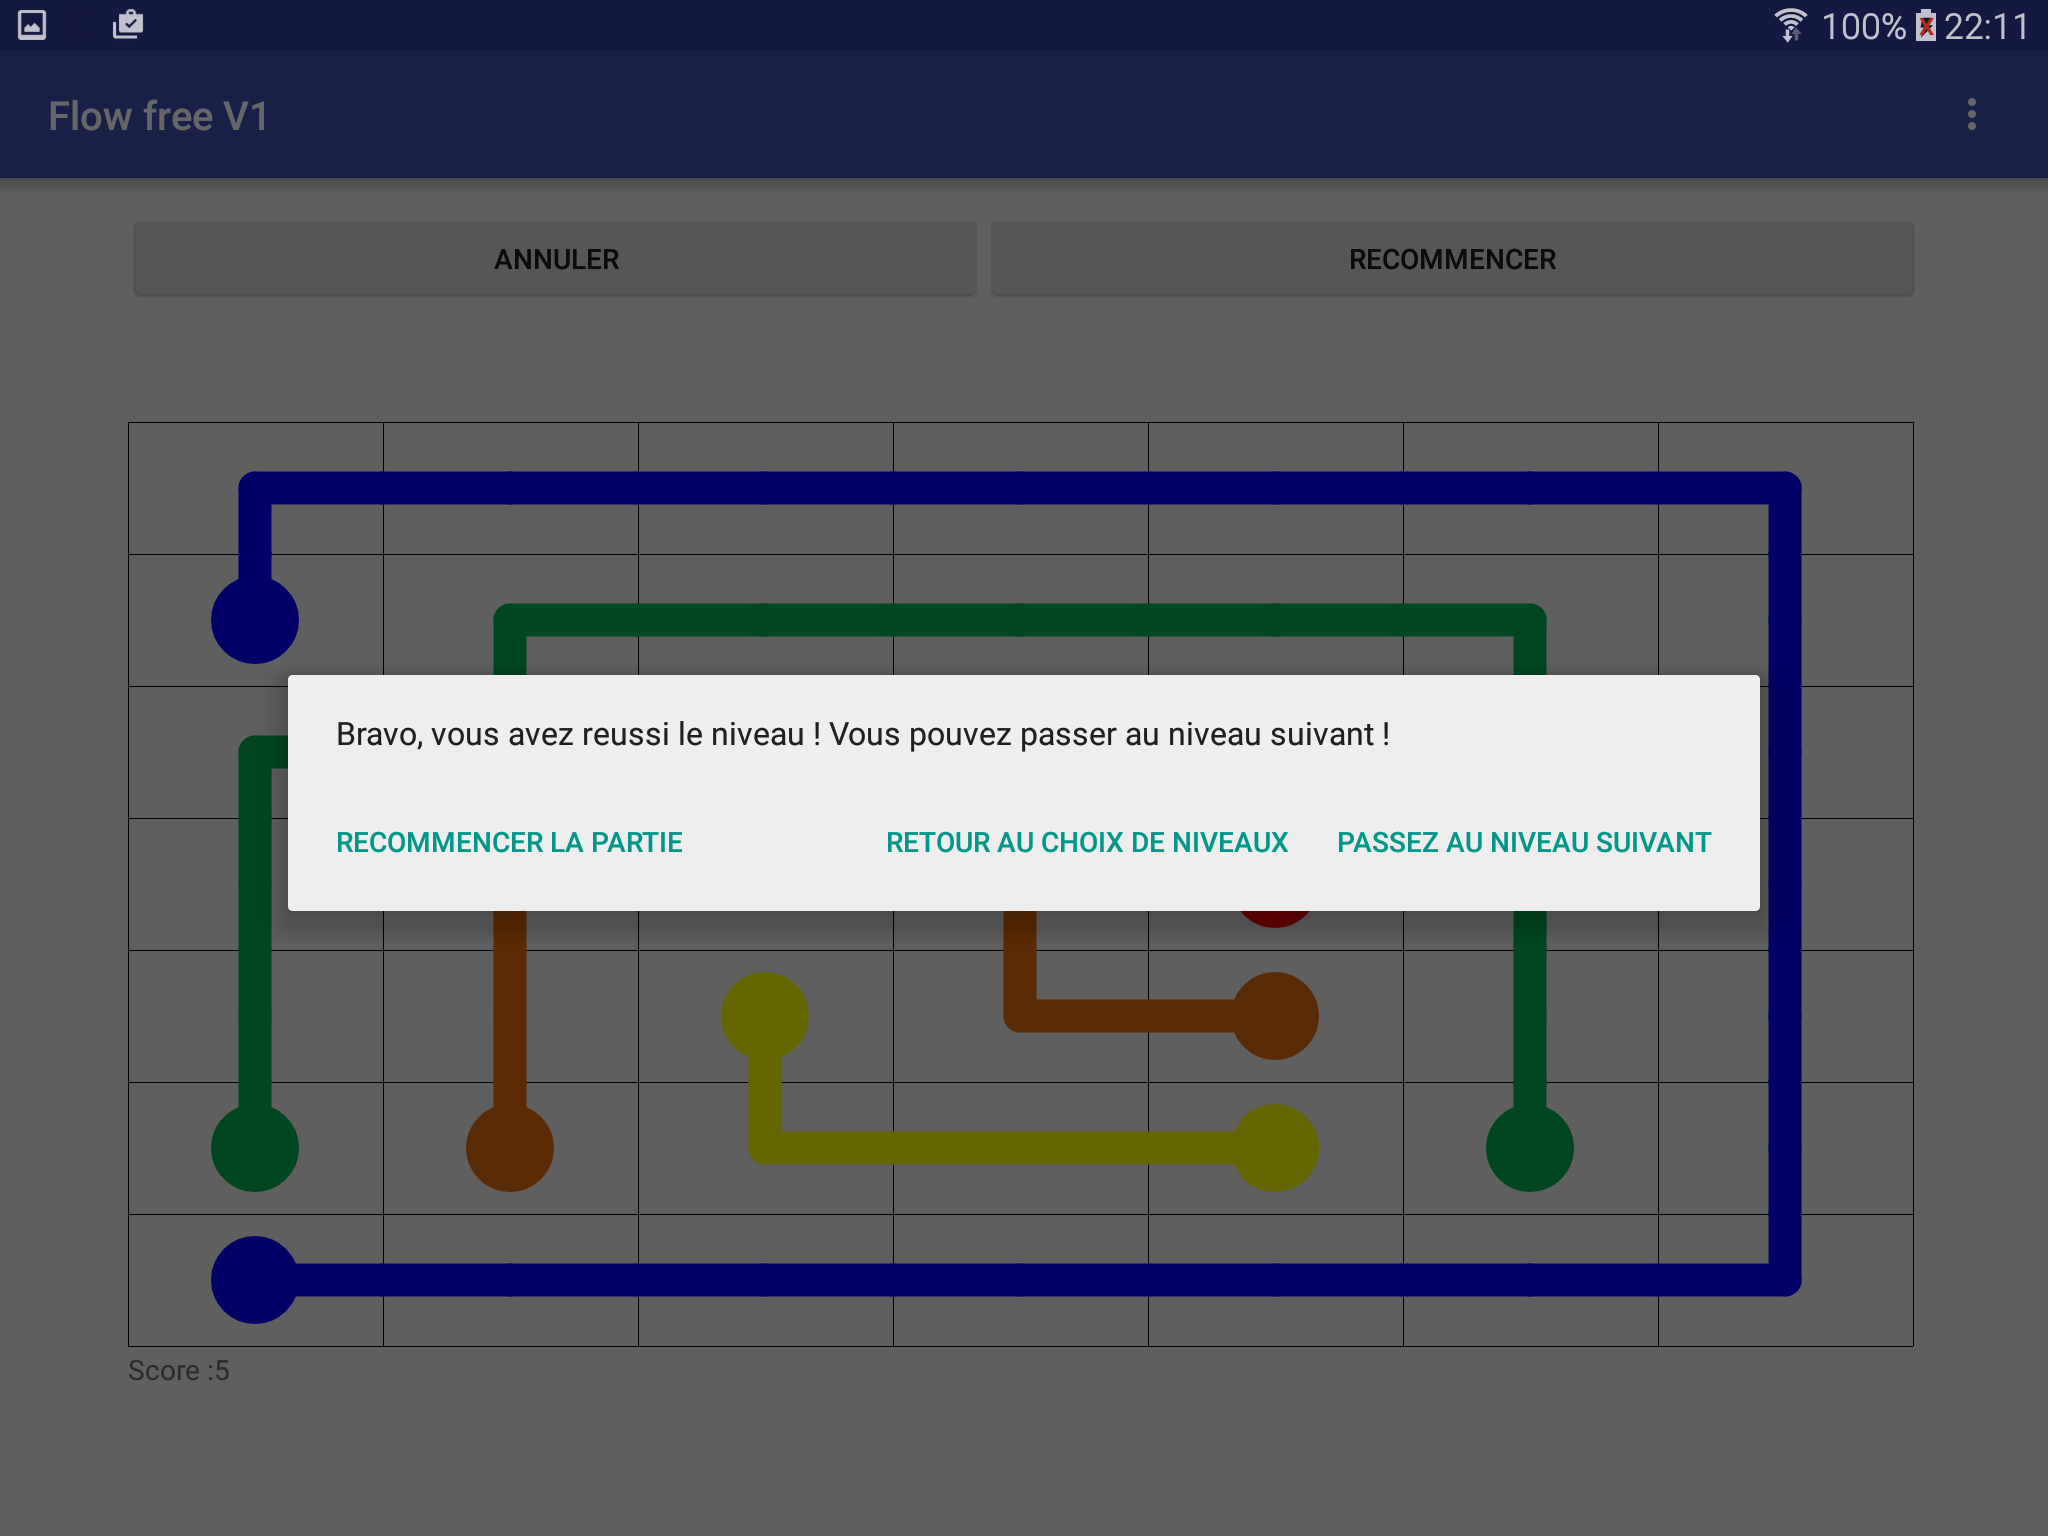
\includegraphics[width=8cm]{Images/s2_4.png}
\caption{Partie en cours et gagnée sur un Samsung Galaxy Tab 2}\label{fig:partie}
\end{figure}
	
	\begin{figure}
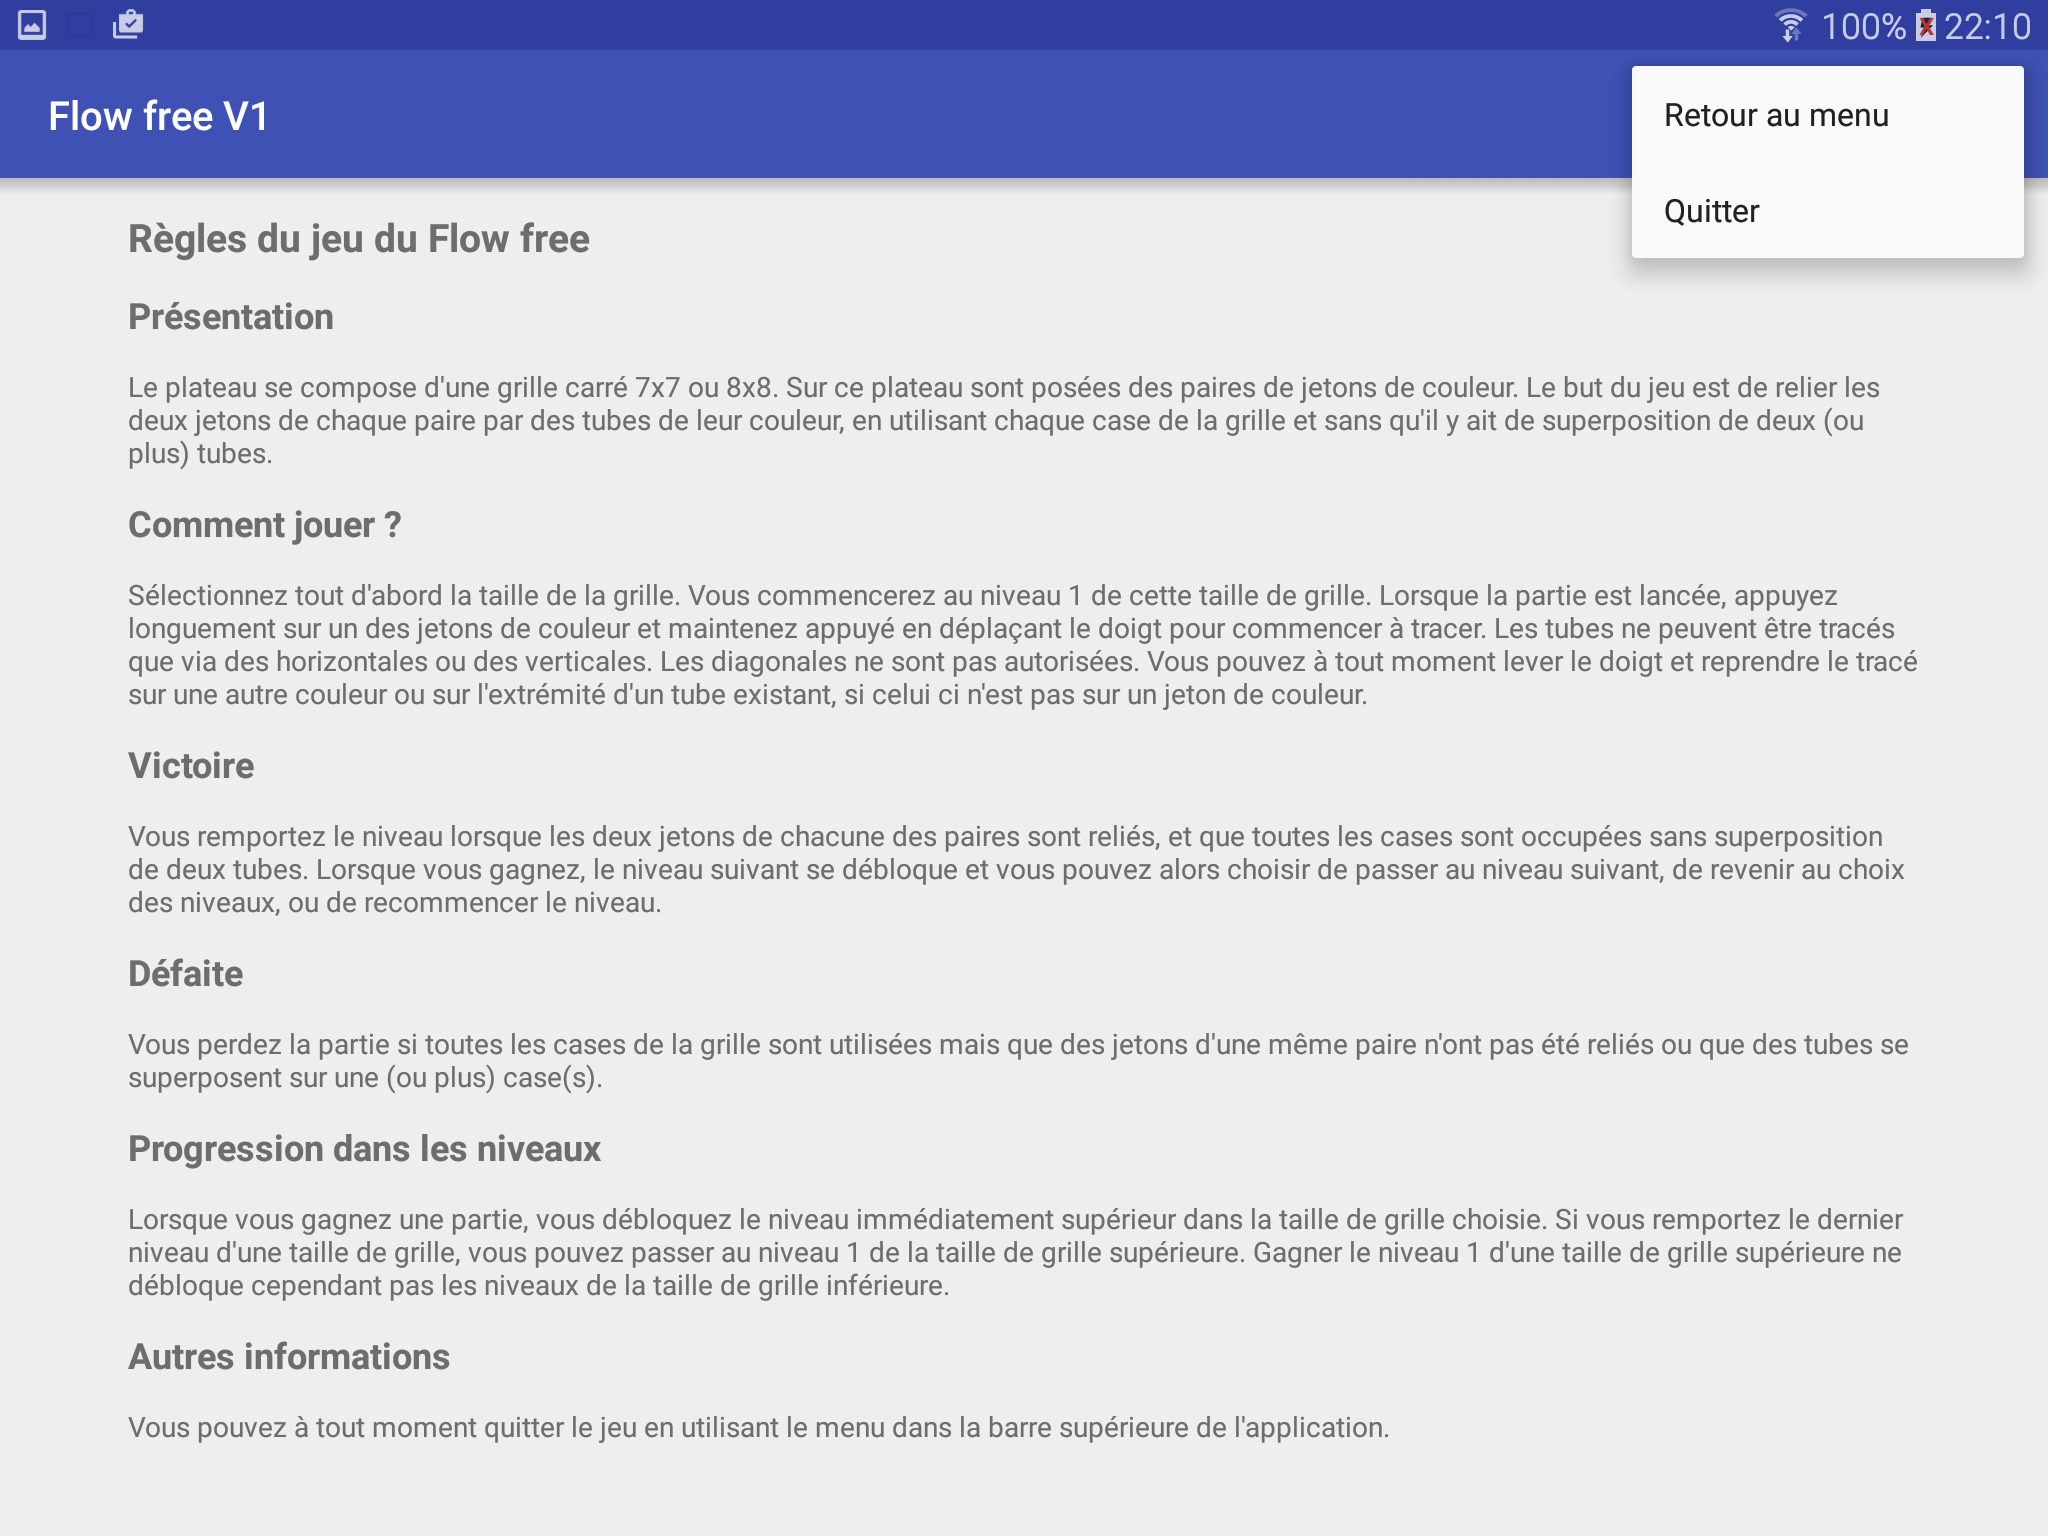
\includegraphics[width=11cm]{Images/s2_2.png}\hfill
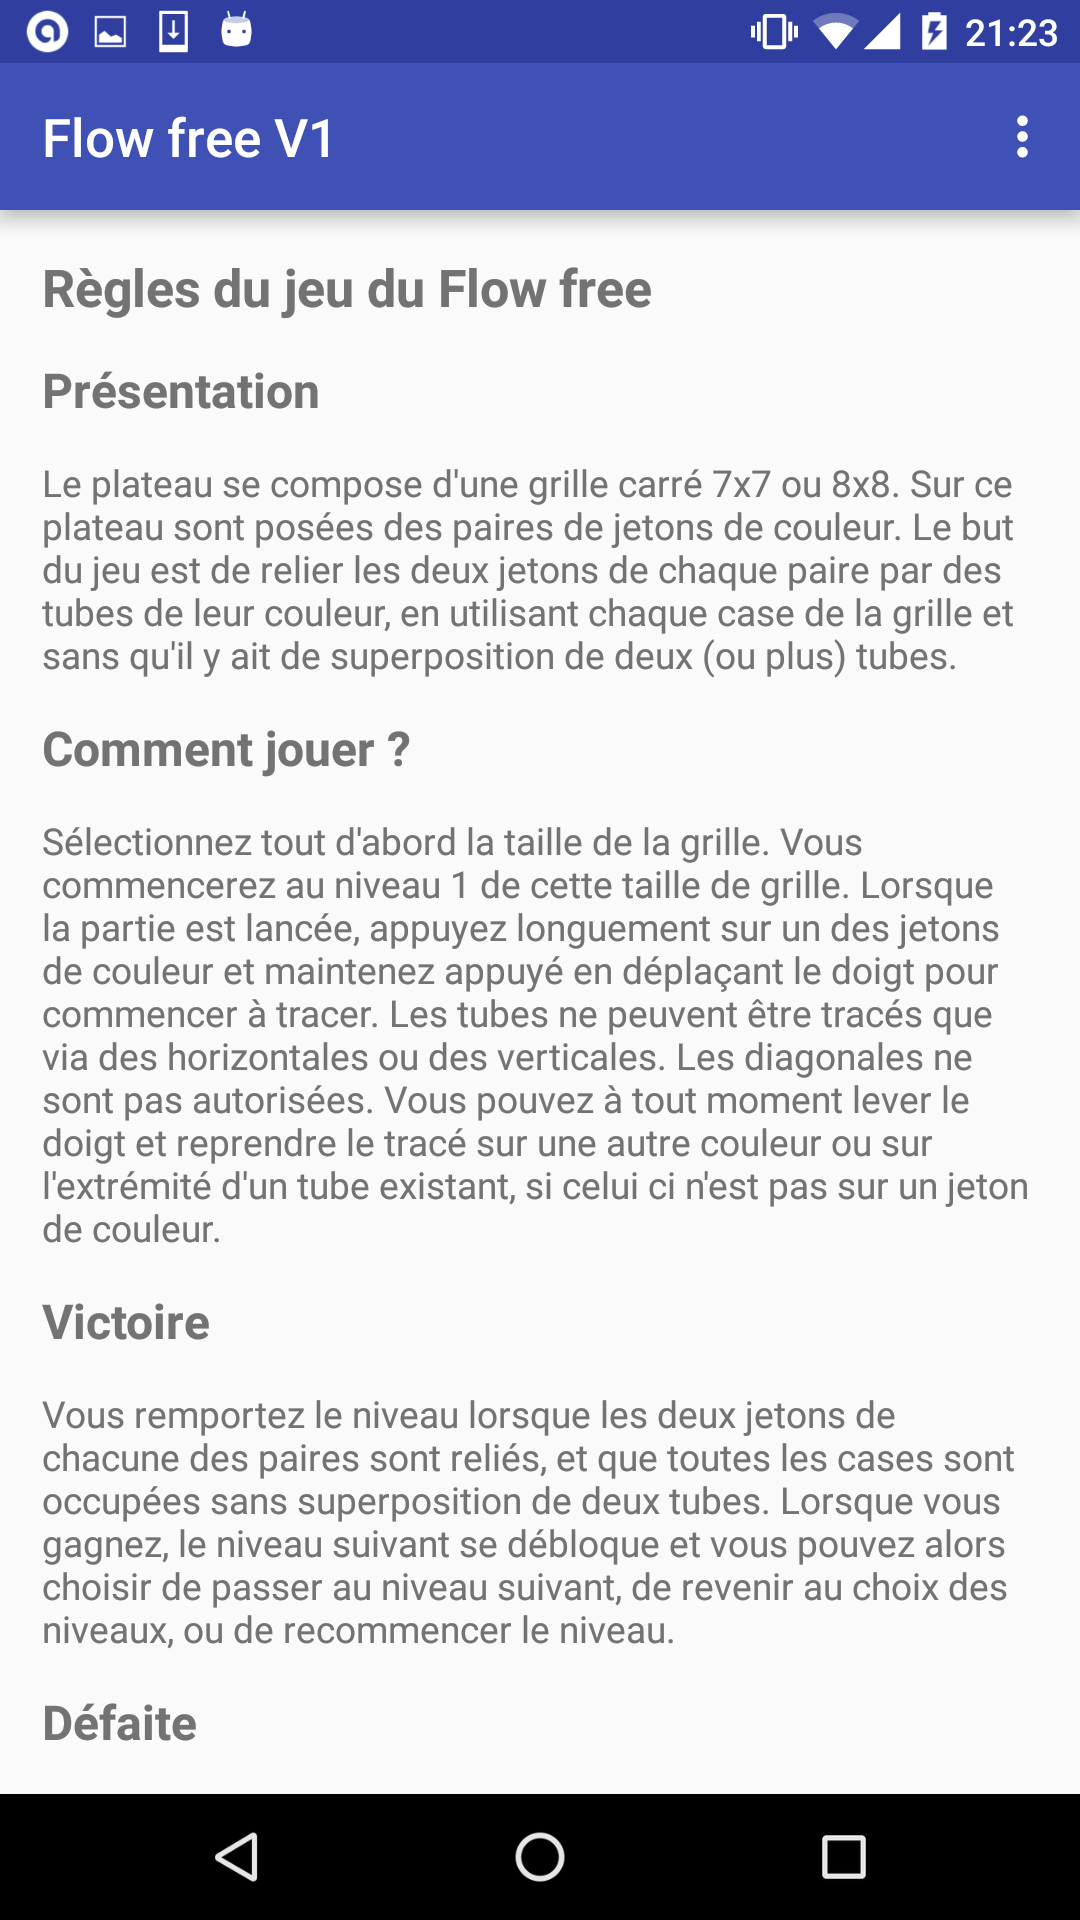
\includegraphics[width=5cm]{Images/nexus_2.png}
\caption{Instructions sur un Samsung Galaxy Tab 2 et Google Nexus 5X}\label{fig:instructions}
\end{figure}

	\subsection{Instructions}
	Pour présenter au joueur des informations utiles à son expérience de jeu, nous avons introduit dans le menu principal un accès aux instructions du jeu. Celle ci sont présentées dans un écran dédié [voir figure \ref{fig:instructions}] , scrollable, et structurées en divers sections, présentant respectivement les règles et mécanismes du jeu, les conditions de victoire, les conditions de défaite, le schéma de progression et de navigation dans les niveaux. Enfin un petit mot est mis sur la possibilité de quitter le jeu via les menus dédiés.
	\newline
	Nous avons vu les principaux choix concernant l'ergonomie et les mécanismes de jeu offerts à l'utilisateur. Dans la section suivante, nous détaillerons les choix techniques effectués pour réaliser l'application.
		 
\section{Présentation Technique}
    \subsection{Affichage de la grille}
    Le dessin se fait en stockant des commandes qui tracent des lignes. Ainsi, nous avons une classe \textit{GridLine} qui
    contient les coordonnées des extrémités d'une ligne, lorsqu'on veut tracer la ligne, on appelle la méthode draw de cette
    classe en lui passant le canvas sur lequel on désire tracer la ligne. Les lignes sont créées lors de l'appel à la méthode
    onSizedChanged afin de connaître les dimensions de la place allouée pour la grille. On divise les dimensions par les
    dimensions de la grille (en nombre de cases). Cela nous donne les dimensions en pixels de chaques cases. On peut alors boucler
    pour tracer une droite à chaque multiple des offset sur les deux axes. Cette droite relirerait deux extrémités (verticales ou
    horizontales).
    \newline

    Les différentes lignes sont alors stockées dans une liste, afin de les parcourir dans la méthode onDraw de la vue, pour
    afficher la grille à chaque action de la part du joueur. Dans cette méthode sont également parcourus l'ensemble des éléments
    de la grille afin de leur demander de se redessiner via leur méthode draw. Ces objets seront détaillés dans la section
    suivante.
    \newline

    Il est important de souligner que l'ensemble des objets grahiques sont créés (ou mis à jour selon les cas) dans la méthode
    onSizedChanged, leurs dimensions sont alors calculées à partir des nouvelles dimensions données par la méthode onSizedChanged
    de ce fait, la grille prendra toujours toute la place possible et les divers objets graphique (ronds, traits) auront toujours
    une bonne dimension adaptée à l'écran du téléphone. Cela permet aussi d'avoir un affichage optimal quel que soit le mode
    (porttrait/paysage) dans lequel est le téléphone.
    \subsection{Fonctionnement de la grille}
    \subsubsection{La grille}
    La grille de jeu est implémentée dans la classe \textit{FlowFreeSimpleGridView}, cette classe étant la classe \textit{View}
afin de posséder toutes les fonctionnalités d'une vue, pour pouvoir intercepter les mouvements de l'utilisateur sur la surface.
Cette vue possèdera un tableau à deux dimensions (nommé grid) représentant les différentes cases de la grille. On distingue deux
types de cases, les cases classiques et les cases contenant un délimiteur. Les cases contenant un délimiteur dans la mesure où,
elles possèdent un cercle de couleur et surtout leur couleur, à tout instant, est toujours du rond présent sur la case. Nous avons
en effet considéré que qu'afin de pouvoir compléter le jeu, que les ronds soit accessibles à tout instant. En effet, dans le cas
contraire, on pourrait se retrouver bloqué dans l'état inachevé car il nous serait impossible de tracer le dernier tube, et donc
d'atteindre l'état de défaite. De ce fait nous voulions pouvoir stoquer deux classes distinctes au sein d'une même structure. De
plus, ces classes on un fonctionnement très proche: elles doivent pouvoir stocker des éléments de tube de couleurs différentes
tout en conservant l'ordre d'arrivée de ces derniers afin de présenter un un affichage cohérent où le dernier morceau de tube
arrivé sur la case serait celui dessiné en dernier (afin que graphiquement il apparaisse au-dessus de l'autre). Il nous a donc
paru naturel de d'utiliser de l'héritage Avec une classe mère AbsGridElement dont héritent deux classes GridElement et
GridDelimiter (qui représente les cases avec un rond de couleur). La classe mère implémente toutes les fonctionalités qui
permettent à une case de contenir un ou plusieurs tubes et de les gérer, tandis que les classes filles implémente la gestion des
couleurs et les opérations à faire en cas de changement de taille (si on passe du mode portrait au mode paysage par exemple).
    \subsubsection{Les élements de la grille}
    Comme il a été dit auparavant, il y a deux catégorie d'éléments ceux avec un délimiteur (un rond de couleur) et ceux sans.
    Chacun de ces deux éléments possède une pile de couleurs, dès qu'un trait de couleur (tube) passe sur la case, la couleur du
    trait est empilée. On stocke alors la position de la partie du tube qui taverse la case dans une hasmap ordonnée
    (couleur->Tube). Ainsi, lorqu'on voudra savoir la couleur courante d'une case, il suffira de vérifier que la pile de couleur
    n'est pas vide, puis de renvoyer le dernier élément de cette pile. Notons que dans le cas des cases ayant un délimiteur, on
    renverra toujours la couleur du délimiteur. Ces deux classes ont également une méthode \textit{draw} qui dessine à l'écran les
    parties de tubes qui passent par la case courante. Les cases ayant un délimiteur traceront également leur rond à ce moment là.
    Les méthodes \textit{updateSize} permettent de mettre à jour les dimensions: dans le cas des délimiteurs, on recalcule le
    rayon du cercle, puis dans les deux cas, on met à jour les coordonnées des parties de tube présent sur la case. (Si la grille
    a changé de taille, les extrémités des tubes doivent être mises à jour).
    \subsubsection{Les tubes}
    Les tubes ont un début et une fin, marqués par un rond. Tant que le joueur n'a pas appuyé sur l'un des ronds, chaque rond est
    susceptible d'être un début de tube ou une fin. Un tube est complété quand les deux extrémités sont reliées. La classe tube
    doit donc posséder les coordonnées de ses extrémités, une couleur et un moyen de savoir quelle extrimité est le début. 
    Cette classe posséde donc deux taleaux l'un pour les délimiteurs, l'autre pour la suite de segments (passage d'un tube à
    l'autre) qui le compose. La classe a également un index, qui détermine le délimiteur choisi comme début de tube.
    Les segments (classe TubPart) sont mis à jour au fur et à mesure que le joueur bouge le doigt sur l'écran.
    Le fait de  stocker les segments (TubPart) dans une liste permet de facilement savoir si le point où le joueur appuie
    correspond bien au dernier élément du tube, ce qui empêche le joueur de tracer un prolongement de tubes depuis une position
    interdite. Cette manière de faire permet également de facilement savoir facilement si le tube est fini.
    \newline

    Sachant que l'utilisateur doit relier tous les ronds entre eux pour pouvoir gagner, et que donc à terme tous les tubes
    existeront, ils sont tous créés lors de l'initialisation de la partie. En revanche, ils seront initialisés, c'est-à-dire que
    le délimiteur qui marque le début sera désigné au moment où l'utilisateur appuiera pour la première fois sur un rond de cette
    couleur. Qui sera alors désigné comme étant le délimiteur de début pour ce tube.
    \subsection{Gestion du tracé}
    Lorsque l'utilisateur appuie sur l'écran, on recupère les coordonnées via l'event, on les divise par la largeur et la longueur
    d'une case via une division entière, cela nous donne les coordonnées de la case sous la forme (i,j). On peut alors directement
    accéder à la case choisie par l'utilisateur en utilisant le fait que les case sont contenues dans un tableau à deux
    dimensions. On met alors à jour le tube correspondant à la couleur actuelle (via la hashmap couleur -> tube). Cette mise à
    jour, passe par la création d'un objet TubPart qui caractérise le fait qu'un tube passe par une case. Cette objet sert de
    conteneur pour deux "morceaux" de tube. (Ces morceaux sont en réalité des segments graphiques reliant le centre de la case aux
    bords de la case suivante et de la case précédente dans le tube). Ainsi, un tube n'est qu'une succession de segment qui sont
    tracés à la suite, la sensation de continuité povient du fait que les extrémités du dit segment se superposent.
    \newline

    Remarque; lors du tracé, il faut vérifier que le mouvement fait par l'utilisateur est cohérent, c'est-à-dire qu'il va sur une
    case à côté de la case de départ, dont la couleur est différente de la case sauf s'il se rend sur le délimiteur qui ferme le
    tube.
    
    \subsection{Gestion des Annulations/Undo}
    Afin de pouvoir fournir au joueur la possibilité d'annuler le dernier mouvement fait, nous avons implémenter une
    fonctionnalité d'annulation. Pour cela nous avons une pile de coordonnées (dans GameState). Ainsi lorsqu'on veut la dernière
    opération, il nous suffit de retirer la dernière position de la pile des coordonnées, récupérer la classe présente à ces
    coordonnées. Lorsqu'on arrive sur cette classe, on peut connaître la dernière couleur qui a été dessinée sur cette case via la
    pile de couleurs contenues dans cette case. Dès qu'on a la couleur, on peut, retirer l'entrée correspondant à cette couleur de
    la hashmap. Il ne reste alors plus qu'à retirer le dernier élément du tube de cette couleur.
    \newline

    Il faut juste, lorsqu'un fait cette opération, prendre garde à garder des scores cohérents, ainsi lorsqu'on quitte une case
    il faut prendre garde à décrémenter le compteur nombre de cases. De même si on vient de supprimer un doublon sur une case.
    De même, si on vient de déconnecter un tube de son dernier délimiteur, il faut le signaler à la logique du jeu afin que l'état
    interne soit cohérent.
    \subsection{Représentation des niveaux}
    Les niveaux ont été représentés dans un fichier XML \textit{levels.xml} situés dans les ressources de l'application (dossier \textit{res/xml}). La structure du fichier XML est la suivante : la racine du fichier est la balise \textit{listOfLevels}, puis au niveau hiérarchique inférieur, on trouve les balises \textit{levelsOfSizeX} (ici X = 7 ou 8) qui permet de regrouper tous les niveaux d'une même taille dans un même niveau hiérarchique. Enfin, chaque niveau est décrit dans une balise \textit{level} avec un attribut \textit{id}.
    \newline
    Plus en détail, chaque niveau dispose de quatre caractéristiques : \textit{unlock}, un booléen qui détermine si le niveau est débloqué ou non en premier lieu, \textit{width} et \textit{height}, respectivement la largeur et la longueur du niveau (en nombre de cases), et enfin un ensemble de composants \textit{listOfComponents}, qui va contenir les informations sur les jetons de départ. Chaque composant (balise \textit{component}) va contenir trois balises et représenter une paire de jetons d'une même couleur : \textit{color} contient bien évidemment la couleur, en hexadécimal ou en littéral. Enfin chacun des deux jetons de couleurs sera représenté par un noeud \textit{circle} qui comprend l'abscisse (\textit{x}) et l'ordonnée (\textit{y}) du jeton dans la grille de départ, la case en haut à gauche étant celle de coordonnées (0,0). Les abscisses sont croissantes vers la droite et les ordonnées vers le bas.
    \newline
    Cette représentation des niveaux présente plusieurs avantages : la structure est assez rigoureusement définie et permet un parsage facile du fichier lors de sa lecture. C'est le mécanisme utilisé d'une part pour déterminer les tailles disponibles dans l'écran de sélection des tailles, ainsi que pour déterminer les niveaux disponibles pour une taille donnée. Ce système étant automatisé, il serait très facile d'ajouter, si on le souhaitait, des niveaux supplémentaires pour les tailles existantes, voire d'ajouter de nouvelles tailles de grille. Ceci rend l'application facilement extensible au besoin, et permet même à des gens qui ne connaissent pas Java ou ne disposent pas du code source de l'application de pouvoir faire du \textit{level-design}.
    
    \subsection{Utilisation des ressources}
    \subsubsection{Utilisation dans l'application}
    Nous avons essayé d'utiliser au maximum le mécanisme des ressources d'Android, notamment en ce qui concerne les \textit{strings}. Ainsi, par exemple, les chaînes de caractères présentées dans les boites de dialogue de confirmation, qui sont communes à toutes les activités, sont définies dans le fichier \textit{strings.xml}, ce qui permet de les changer facilement. De même, les textes des différents boutons du menu principal sont définis dans ce même fichier.
    Nous avons également utilisé les ressources bien évidemment pour les layouts, qui sont relativement simples mais répondent bien aux caractéristiques que nous voulions avoir, ainsi que pour définir une icône pour l'application, qui est celle présentée sur la page de garde.
     
     \subsubsection{Cas particulier des instructions}
     Les instructions ont représenté un cas particulier dans l'utilisation des ressources. Nous avons hésité entre deux approches, l'une consistant à créer différents paragraphes via des \textit{TextView}, avec certains d'entre eux ayant un style particulier pour représenter les titres de section. Nous avons préféré opté pour l'autre solution et tirer partie des possibilités offertes par Android d'utiliser du texte formaté en HTML. Nous avons donc défini, dans le fichier \textit{strings.xml}, une string un peu particulière, comprenant du HTML. Pour que celle-ci soit reconnue en tant que telle, il a fallu entourer son contenu (l'intérieur de la balise <string>), par \textbf{<![CDATA[} \textit{HTML} \textbf{]]>}, et transmettre cette valeur à la méthode \textit{Html.fromHtml} dans l'\textit{InstructionsActivity}, pour que le HTML soit parsé. L'objet \textit{Spanned} récupéré a ensuite pu être transmis à la méthode \textit{setText} du \textit{TextView}, que l'on a d'ailleurs rendu \textit{scrollable}.
      
  \subsection{Navigation entre les activités}
  	Chaque activité dans notre application va contenir une a plusieurs vues, c'est dans ces vues que nous représentons les différents éléments du jeu, comme les boutons de navigations dans le jeu, la grille de jeu, etc... Une activité a un rôle particulier, nous allons nous intéresser aux activités qui nous permettent de jouer au jeu demandé :
  	\begin{itemize}
  	\item La MainActivity représente l'activité principale du jeu, c'est elle qui va afficher le menu de départ du Flee Flow et qui va nous permettre de choisir différentes possibilités comme Démarrer le jeu, voir les instructions du jeu ou simplement quitter le jeu.
  	\item Une fois le jeu lancé, nous passons à l'activité ChooseSize, va nous permettre de choisir quelle est la taille de grille avec laquelle nous désirons jouer, soit du 7x7 soit du 8x8.
  	\item Dès que nous cliquons sur la taille souhaitée pour la grille de jeu, l'activité ChooseSize va nous donner la possibilité de choisir le niveau de difficulté (de 1 à 3), en sachant qu'à la première partie que nous allons faire après le lancement, nous n'avons la possibilité de jouer qu'au niveau 1 de la grille 7x7 et du niveau 1 de la grille 8x8.
  	\item Le niveau de jeu choisi, nous pouvons désormais jouer une partie. Après la génération de l'activité InGame, nous avons la grille de jeu avec les jetons délimiteurs à joindre qui apparaissent aux endroits demandés selon le niveau. Nous avons aussi l'apparition dans la vue de deux boutons, un bouton Annuler qui permet de revenir au coup précédent, et un bouton Recommencer qui va faire revenir notre grille dans son état de départ.
  	\end{itemize}
Lors du déroulement de notre Flee Flow, nos différentes activités qui sont impliqués dans la génération et la gestion de la grille de jeu vont devoir communiquer. En effet dès la Main Activity, nous récupérons les différents niveaux selon la taille de la grille depuis le fichier XML levels.xml. Nous allons stocker ces informations dans une première entité globale représentée par la classe LevelsBySize, contenant toutes les informations nécessaire à la génération des différentes grilles. Les informations vont être transmises de l'activité créatrice et l'activité générée, grâce à un objet Intent, ces informations vont être utiles pour la bonne continuation du jeu. Ainsi la Main Activity va transmettre les informations pour afficher correctement les deux boutons de choix de tailles de la grille. \'A partir de la notre activité de choix de taille va prendre les données nécessaires et choisir celles utiles pour l'activité suivante, nous allons passer comme données des Levels(classes nous permettant de savoir comment doivent être générées les bonnes grilles), et les niveaux qui sont débloqués.
La classe ChooseLevel va représenter tous les niveaux disponibles tout en empêchant de sélectionner les niveaux qui n'ont pas été débloqués comme demandé dans l'énoncé du TP. Une fois le niveau selectionné, nous transmettons les informations du niveau avec un objet level, et l'identifiant de ce niveau. La partie à jouer pourra ainsi être simplement affiché.

Nous voyons donc l'importance de la communication d'une activité à une autre. Mais pour permettre le retour en arrière, par exemple si le joueur veut changer de niveau, ou il voudrait revenir dans un niveau de sélection du jeu précédent, nous devons nous souvenir de certaines informations. C'est pourquoi nous avons choisi de créer des activités mais aussi d'attendre un retour de l'activité créée avec la fonction StartActivityForResult. Cela nous permet de retransmettre les informations reçus par l'activité précédente, mais mise à jour. Nous pouvons ainsi naviguer aisément dans notre jeu, choisir les niveau, mais aussi revenir en arrière tout en conservant les informations de notre partie actuelle. Cependant, comme nous ne stockons pas d'informations dans un fichier de sauvegarde, une fois que nous avons quitté le jeu, au redémarrage, nous repartons avec les configurations initiales, c'est-à-dire que nous n'avons que le niveau 1 des deux différentes tailles de grille qui sont accessibles.  

\section{Difficultés rencontrées}
  \subsection{La compréhension d'android}
  Le sujet qui nous a été proposé est très intéressant pour découvrir les fonctionnalités de base des applications Android. Nous avons pu mettre en œuvre la mise en place de vues dans une activité, les dialogues entre les vues et l'activité, etc...
  
L'une des difficultés principales que nous avons eu lors du déroulement de notre projet a été de découvrir et de s'approprier les connaissances nécessaires à la bonne implémentation du jeu qui nous avait été demandé. En effet, Android étant aujourd'hui une plateforme très populaire, nous avons la chance de pouvoir accéder à de très nombreuses ressources et documentations sur les bases pour comprendre le développement sous android. Cependant nous avons aussi été face à la difficulté de trouver la bonne documentation pour ce que nous souhaitions réaliser. Et comme nous étions novices dans la programmation Android, et même pour certains peu connaisseurs du langage JAVA, cela nous a pris un peu de temps pour maîtriser les bases nécessaires pour obtenir une première version fonctionnelle du Flee Flow. 
Lors de la phase d'implémentation de notre jeu, nous avons longtemps hésité entre utiliser des fichiers de sauvegarde pour mémoriser les informations sur la partie de l'utilisateur ou transmettre les données entre les activités, comme il a été finalement choisi. Il a été difficile de prendre en main correctement la transmission correcte entre une vue et une activité. C'est notamment ce qui nous a fait hésité à utiliser un fichier de sauvegarde annexe. Mais nous avons pu découvrir par une utilisation judicieuse des méthodes (startActivityOnResult, OnActivityResult) que nous pouvions communiquer assez aisément entre les différents éléments de notre application. Ce point a été le plus difficile à mettre en place, notamment sur les données à conserver entre chaque communication, et nous a pris un temps non-négligeable, ce qui ne nous a pas permis d'accentuer un peu plus nos efforts sur l'aspect graphique du jeu. Ce choix a posteriori de notre méthode communication entre les différents éléments a été donc difficile à mettre en place avec la structure que nous avions choisi pour représenter les différents éléments de la grille de jeu (Les tubes, les parties de tubes, les jetons délimiteurs,...). 
Nous avons aussi choisi pour une utilisation plus aisé du jeu, d'introduire un bouton undo, qui permet au joueur d'effacer la dernier portion de tube entre les deux dernières cases qu'il a touché. Cet ajout bien que non demandé, mais qui pour nous donne une plus grande maniabilité à notre jeu, étant donné que le joueur n'a plus à recommencer entièrement sa partie, a demandé une modification assez conséquente de notre structure pour inclure un stockage des différentes actions de l'utilisateur et le "bon retour" en arrière pour que le jeu soit toujours fonctionnel, et qu'il n'y ait pas de bugs dans la suite du déroulement de la partie.
  \subsection{Le travail en équipe}
La premier difficulté dans un tel projet est le travail en groupe, il est essentielle de se mettre d'accord sur les bases que nous voulons pour notre projet. Nous avons essayé de mettre en place un squelette sur lequel nous baser pour créer la structure de notre projet. Mais ayant des points de vue différents, nous avons mis du temps à trouver un accord sur ce que nous pensions chacun comme bon pour l'implémentation du jeu. Il nous a donc fallu du temps pour nous mettre d'accord sur l'architecture et les différentes classes que nous avons utilisé. Il est aussi arrivé que nous faisions des erreurs dans la compréhension du code implémenté par une autre personne du groupe.
Comme nous découvrions la programmation pour application mobile Android, nous avons essayer de répartir au mieux les tâches pour que chacun puisse en apprendre le plus possible. Par ce fait, nous étions plus dépendants les uns des autres, ce qui a notamment demandé plus de temps dans l'intégration des différents composants implémentés par chacun. 

  \subsection{Le temps}
  Lors de ce projet, nous avons fait de nombreuses modifications par rapport à ce que nous avions convenu au départ. Ces changements, et la formation nécessaire pour pouvoir nous permettre de réaliser ce que nous voulions nous a empêcher de terminer tous les points que nous nous étions fixés. Nous avons notamment décidé de simplifier notre partie graphique, nos différents essaies sur la mise en place notamment de boutons personnalisés, ou d'image-boutons, n'ont pas été assez fructueuses pour que nous les intégrions à l'application qui a été remise. Nous avons manqué de temps pour gérer le bon dimensionnement des images lors du passage du mode portrait au mode paysage. 
  Nous avons trouvé par ailleurs difficile, de placer comme nous voulions les différents layout et les différents éléments dans ceux-ci. Il serait notamment intéressant d'avoir des fichiers exemples fournis pour la réalisation du TP. Enfin, nous avons mal jugé le temps que nous prendrait le design de notre application. Nous avons sûrement sous-estimé la difficulté de placer et de dimensionner les éléments dans l'interface graphique.

 
  \subsection{Répartition des tâches}
  Un défi majeur de ce TP aura été la répartition des tâches, en effet, une grosse partie du travail était au niveau de la grille,
  de ce fait la personne ayant réalisé la grille aura de grandes chances de devoir faire le reste: gestion des mouvements, tests
  de victoire, etc...
  On peut donc se retrouver avec une disproportion de la charge de travail selon la personne. De plus, cela est frustrant pour les
  autres car il leur est diffile de se trouver une place, de contribuer et de s'exécer à la programmation android.
\section{Critiques et suggestions}
  \subsection{Le Code}
  \'A l'issue de ce tp, nous avons un programme fonctionnel, toutefois, il nous semble que notre programme est plus compliqué que
  nécessaire. L'utilisation de deux arrayList dans les Tube, est totalement inutile est complique la compréhension ainsi que
  l'ajout de fonctionnalités.
  \newline

  De plus la répartition des tâches est assez disproportionnée, nous avons une classe GridSimpleview qui possède la quasi totalité
  de la logique de l'application, ce qui induit un code long, lourd et donc compliqué à comprendre. Il aurait été préferrable de
  découper davantage en sous-classes. Par ailleurs, un découpage en plusieurs paquetages aurait pu être envisagé, nottamment pour
  les classes servant d'utilitaire pour faciliter l'implémentation de parcelable d'en d'autre classes. ce qui aurait grandement
  simplifié la compréhension du code.
\end{document}
